%\myChapter{Titre}{Titre court}
\myChapter{Domain Name System and  Machine Learning}{}{}
%\myMinitoc{Profondeur de la minitoc (section|subsection|subsubsection)}{Titre de la minitoc}
\myMiniToc{}{Contents}

%\mySectionStar{Titre}{Titre court}{Ajouter à la table des matières? (false|true|chapter|section|subsection|subsubsection -section par défaut-)}
\mySection{Introduction}{}
The Domain Name System (DNS) is a hierarchical and decentralized naming system for devices connected to the internet or a private network. It translates human-friendly domain names like www.example.com into IP addresses like 192.0.2.1 that computers use to identify each other on the network. Without DNS, users would need to remember and use IP addresses to access websites or online services. In the other hand,artificial intelligence (AI) is the simulation of human intelligence processes by machines, especially computer systems. These processes include learning (the acquisition of information and rules for using the information), reasoning (using rules to reach approximate or definite conclusions), and self-correction. AI encompasses a variety of subfields and techniques aimed at enabling machines to perform tasks that typically require human intelligence. A major sub field of AI is Machine Learning (ML), which focuses on the development of algorithms that allow computers to learn from and make predictions based on data. Machine Learning is divided into several categories which ware going to be discussed later in this chapter.

\begin{figure}[ht!]
	\centering
	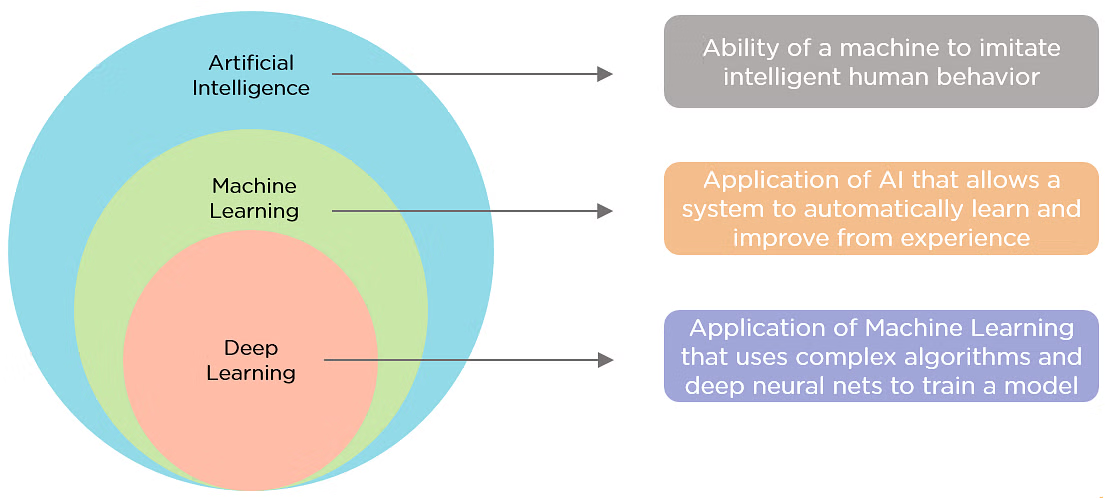
\includegraphics[width=0.9\linewidth]{Chap1/images/MLvsDLvsIA}
	\caption{The domains of {AI} \cite{shruti2023aivs}.}
	\label{fig:mlvsdlvsia}
\end{figure}
\mySection{Overview of DNS}{}
The Domain Name System (DNS) is an essential component of the internet infrastructure, functioning as the internet's directory. DNS translates human-friendly domain names like www.example.com into numerical IP addresses like 192.0.2.1 that computers use to identify each other on the network. This process is crucial because, while domain names are easy for people to remember, computers use IP addresses to locate and communicate with each other.

\subsection{Basic concepts}
\begin{enumerate}
	\item Domain Names:  A domain name is a string that identifies a realm of administrative autonomy, authority, or control on the internet. Examples include example.com, openai.com.
	
	\item IP Addresses: These are numerical labels assigned to each device connected to a computer network that uses the Internet Protocol for communication. They serve two main functions: identifying the host or network interface and providing the host's location.
\end{enumerate}
\subsection{DNS hierarchy:}
The DNS is organized in a hierarchical structure:

\begin{itemize}
	\item Root Level: The top of the DNS hierarchy, represented by a dot (.). It contains information that points to the top-level domain (TLD) servers.
	
	\item Top-Level Domains (TLDs): These are the highest level of domain names in the root zone. Common TLDs include .com, .org, .net, as well as country code TLDs like .uk, .jp.
	\item Second-Level Domains: These are directly below TLDs and are typically what people purchase from domain registrars (e.g., example in example.com).
	\item Subdomains: These are domains that are part of a larger domain (e.g., blog.example.com where blog is a subdomain of example.com).
\end{itemize}
\subsection{DNS-components}
\begin{itemize}
	\item DNS Resolvers: These are responsible for initiating and sequencing the queries that lead to a full resolution of the requested resource, usually managed by ISPs or enterprise networks.\\
	\item Root Name Servers: These servers know where to direct queries for each top-level domain (TLD).\\
	\item TLD Name Servers: These servers store information for each domain within the TLD and direct queries to the appropriate authoritative name servers.\\
	\item Authoritative Name Servers: These servers contain the actual DNS records for a domain and provide answers to queries about those records.
\end{itemize}
\subsection{DNS records:}
DNS records are used to store data about domain names. Key types include:\\

\begin{itemize}
	\item A Record: Maps a domain to an IPv4 address.\\
	\item AAAA Record: Maps a domain to an IPv6 address.\\
	
	\item CNAME Record: Canonical Name record; maps an alias domain name to the canonical domain name.\\
	\item MX Record: Mail Exchange record; specifies the mail server responsible for receiving email for the domain.\\
	\item NS Record: Name Server record; indicates which DNS server is authoritative for that domain.\\
	\item PTR Record: Pointer record; used for reverse DNS lookups to map an IP address to a domain name.\\
	\item TXT Record: Text record; used to store arbitrary text data, often for verification and security purposes.
\end{itemize}

\textbf{How DNS works\\}

Lets Consider the following figure:


\begin{comment}
	
	\begin{figure}[ht!]
		\centering
		\includegraphics[width=0.8\linewidth]{image dns good.png}
		\caption{How DNS resolution works \cite{cloudflare2023dns}}
		\label{fig:enter-label1}
	\end{figure}
\end{comment}

\begin{figure}[ht!]
	\centering
	\includegraphics[width=0.8\linewidth]{chap1/images/image dns good.png}
	\caption{how dns resolution works}
	\label{fig:enter-labeel1}
\end{figure}

\section*{How DNS Works}
Lets consider the workflow of DNS in  FIGURE \ref{fig:enter-label1} where a user enters a url through his or her web browser till when obtained the corresponding ip address. Lets explains detailly the scenario from ppoint 1 to 13: 
\begin{enumerate}
	\item \textbf{Query for the iP address:} When a user types a URL (e.g., http://mypage.com) into their web browser, the process of resolving the domain name to an IP address begins.
	
	\item \textbf{Local cache check:} The first step is to check if the IP address is stored in the local cache, which includes the browser cache, OS cache, and router cache. If the IP address is found here, the process stops, and the website is loaded from the cached IP address. If not, it moves to the next step.
	
	\item \textbf{Host files:} If the IP address is not found in the local cache, the system checks the host files. These files can manually map domain names to IP addresses. If the IP address is found in the host files, the process stops, and the website is loaded.
	
	\item \textbf{DNS resolver query:} If the IP address is not found in the local cache or host files, the query is sent to the DNS resolver, also known as a recursive resolver. This resolver is typically provided by the user's Internet Service Provider (ISP).
	
	\item \textbf{Root server query:} The DNS resolver then queries a root server. There are 13 sets of root servers worldwide, and they contain information on top-level domain (TLD) servers (such as .com, .org, .net).
	
	\item \textbf{TLD server query:} The root server responds with the address of a TLD server responsible for the queried domain. For example, if the query is for a .com domain, the root server provides the address of the .com TLD server.
	
	\item \textbf{Authoritative name server query:} The DNS resolver then queries the TLD server for the authoritative name server that holds the actual DNS records for the domain (mypage.com in this case).
	
	\item \textbf{Domain Nameserver Query:} The TLD server responds with the address of the domain's authoritative nameserver.
	
	\item \textbf{Authoritative nameserver response:} The DNS resolver queries the authoritative nameserver for the specific IP address of the domain (mypage.com).
	
	\item \textbf{IP address response:} The authoritative nameserver responds with the IP address of the requested domain.
	
	\item \textbf{Local cache update:} The DNS resolver stores the IP address in its local cache for future queries. This helps speed up the resolution process for subsequent requests for the same domain.
	
	\item \textbf{Query completion:} The DNS resolver sends the IP address back to the user's computer.
	
	\item \textbf{Website access:} With the IP address obtained, the user's computer can now contact the real server hosting the website (mypage.com) and load the webpage.
\end{enumerate}



\subsection{DNS anomalies}
Anomalies are patterns in data that deviate from the expected norm, arising from various abnormal activities such as credit card fraud, mobile phone fraud, and cyberattacks. These deviations are crucial for data analysts to identify. One important aspect of anomaly detection is understanding the nature of the anomaly, which can be categorized as follows:\\

\subsubsection{ Point anomaly}
When an individual data instance significantly deviates from the typical pattern of the dataset, it is identified as a point anomaly. For instance, if a person typically uses five liters of fuel per day for their car but suddenly uses fifty liters on a random day, this would be considered a point anomaly.

\subsubsection{ Contextual anomaly}
This type of anomaly occurs when a data instance is anomalous within a specific context, also known as a conditional anomaly. For example, credit card expenditures tend to be higher during festive periods such as Christmas or New Year. While high spending is normal for these contexts, it might be anomalous at other times of the year. Conversely, equally high expenditure during a non-festive month could be deemed a contextual anomaly.

\subsubsection{ Collective anomaly}
When a collection of similar data instances behaves anomalously with respect to the entire dataset, the group of data instances is termed a collective anomaly. For example, in a human's Electrocardiogram (ECG) output, the existence of low values for a long period of time indicates an outlying phenomenon corresponding to an abnormal premature contraction, whereas one low value by itself is not considered anomalous.
\subsubsection{ Seasonal anomaly}
Deviations from expected seasonal patterns. For instance, an unexpected spike in electricity consumption during a typically low-demand season could be a seasonal anomaly.

\subsubsection{ Spatial anomaly}
Anomalies that occur in a specific spatial context. For example, unusual traffic congestion in a normally low-traffic area could indicate a spatial anomaly.

\subsubsection{ Behavioral anomaly}
When an entity behaves differently than its usual pattern. For example, a user's sudden change in login times or locations could be considered a behavioral anomaly.
\subsection{DNS Attacks}
DNS attacks exploit vulnerabilities in the DNS protocol and infrastructure to disrupt normal operations or intercept data.

\subsubsection{Man-in-the-middle (MitM) attack}
\textbf{Overview\\}
In a MitM attack, the attacker secretly intercepts and relays messages between two parties who believe they are communicating directly with each other.\\

\begin{figure}[ht!]
	\centering
	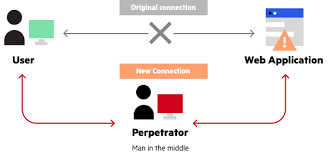
\includegraphics[width=0.5\linewidth]{chap1/images/man in the middle.png}
	\caption{Man in the middle attack \cite{howstuffworks2023dns}}
	\label{fig:enter-label}
\end{figure}


\textbf{How it Works}
\begin{enumerate}
	\item \textbf{Interception:} The attacker intercepts the communication channel between the client and the DNS server.
	\item \textbf{Relay:} The attacker can modify or eavesdrop on the messages.
	\item \textbf{Consequences:} This can lead to data theft, insertion of malicious content, or redirection to fake websites.
\end{enumerate}

\subsubsection{DNS Spoofing (DNS Cache Poisoning)}
\textbf{Overview\\}
DNS Spoofing, or DNS Cache Poisoning, involves corrupting a DNS server's cache with false information.


\begin{figure}[ht!]
	\centering
	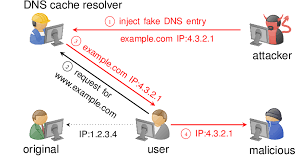
\includegraphics[width=0.5\linewidth]{chap1/images/cache poisning.png}
	\caption{Cache poisoning \cite{datadog2023dns}}
	\label{fig:enter-label}
\end{figure}


\textbf{How it Works}
\begin{enumerate}
	\item \textbf{Injection:} The attacker sends forged DNS responses to a DNS resolver.
	\item \textbf{Poisoning:} These false responses are cached by the DNS resolver.
	\item \textbf{Redirection:} Future queries for the poisoned domain are directed to the attacker's IP address.
	\item \textbf{Consequences:}
\end{enumerate}


Users can be redirected to malicious websites designed to steal information or infect devices with malware.

\subsubsection{DoS and DDos attacks}
A DoS attack aims to make a DNS server unavailable by overwhelming it with a large number of requests. In the other hand,a DDoS attack is a more powerful form of DoS, where multiple systems (often part of a botnet) are used to flood the DNS server with traffic.
\begin{figure}[ht!]
	\centering
	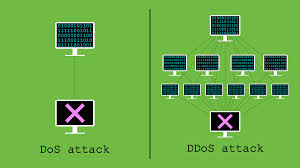
\includegraphics[width=0.5\linewidth]{chap1/images/dos.jpg}
	\caption{DoS and DDoS attack \cite{liquidweb2023dns}}
	\label{fig:enter-label}
\end{figure}

\textbf{How it Works}
\begin{enumerate}
	\item \textbf{Flooding:} The attacker sends a high volume of requests to the DNS server.
	\item \textbf{Overloading:} The server becomes overwhelmed and cannot process legitimate requests.
\end{enumerate}

\textbf{Consequences:}
Legitimate users are unable to resolve domain names, leading to service disruption.

\subsubsection{DNS Tunneling}

\textbf{Overview\\}
DNS Tunneling exploits DNS to tunnel malware and other data through a network firewall.

\begin{figure}[ht!]
	\centering
	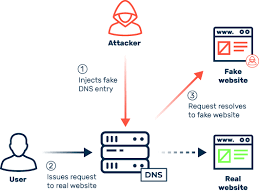
\includegraphics[width=0.5\linewidth]{chap1/images/dns spoofing.png}
	\caption{DNS tunneling \cite{cloudacademy2023dns}}
	\label{fig:enter-label}
\end{figure}

\textbf{How it Works}
\begin{enumerate}
	\item \textbf{Encoding Data:} Data is encoded into DNS queries.
	\item \textbf{Transmission:} These queries are sent to an external server controlled by the attacker.
	\item \textbf{Decoding Data:} The external server decodes the data from the DNS queries.
\end{enumerate}

\textbf{Consequences}
This technique can be used to exfiltrate sensitive information or establish command and control channels for malware.

\subsubsection{Cache Poisoning}
\textbf{Overview\\}
Cache poisoning is a specific type of DNS Spoofing that targets DNS caches, causing them to store incorrect information.

\begin{figure}[ht!]
	\centering
	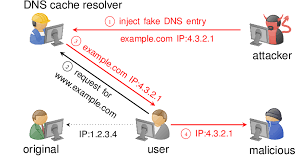
\includegraphics[width=0.5\linewidth]{chap1/images/cache poisning.png}
	\caption{cache poisonning\cite{datadog2023dns}}
	\label{fig:enter-label}
\end{figure}
\textbf{How it Works\\}
\begin{enumerate}
	\item \textbf{Forged Responses:} The attacker sends forged DNS responses to the DNS server.
	\item \textbf{Cache Storage:} These forged responses are stored in the DNS server's cache.
	\item \textbf{Misdirection:} Subsequent queries for the poisoned domain are directed to the attacker's IP address.
\end{enumerate}
\textbf{Consequences:}
Similar to DNS Spoofing, users are redirected to malicious sites, facilitating phishing, malware distribution, and other attacks.


\mySection{Types of Artificial Intelligence}{}

Artificial intelligence, so far, represents the ability of a program or a machine to solve complex problems by imitating human cognitive processes. It is also capable of performing intellectual tasks at a level often superior to humans in most cognitive domains. There are mainly two types of AI: strong artificial intelligence (AGI or strong AI) and weak artificial intelligence (weak AI).



\mySubSection{Weak Artificial Intelligence}{}

Weak AI, also called narrow AI, focuses on solving specific tasks, such as solving chess problems. Unlike general AI, this type of artificial intelligence does not exhibit creativity or the ability to learn autonomously in a universal way.\\ Its learning capabilities rely on pattern detection (machine learning) or comparing large amounts of data. The benefits of weak AI are particularly notable in automation and process control, as well as in speech recognition and processing. Among its applications are text and image recognition, speech recognition, text translation, and navigation systems, among others.
\mySubSection{Strong or General Artificial Intelligence}{}
General AI represents an artificial intelligence model designed to surpass human cognitive abilities in almost every field. Unlike weak AI, which is limited to specific tasks, general AI has the ability to analyze, interpret, and solve complex problems that arise in daily life. This includes advanced creativity skills, a deep and nuanced understanding of human emotions, and the ability to make autonomous decisions and move independently.
This form of AI could, for example, compose original music, write novels, or diagnose diseases with greater accuracy than the best human experts. It could also interact empathetically with humans, understand their emotional needs, and respond appropriately, while performing complex physical tasks without supervision \cite{elboudkhani2019}.
However, implementing general AI requires considerable investments in several areas. This includes massive financial resources for research and development, advanced computing infrastructures to manage large-scale data processing and storage, and a highly skilled workforce to design, program, and maintain these complex systems.

\begin{figure}[ht!]
    \centering
    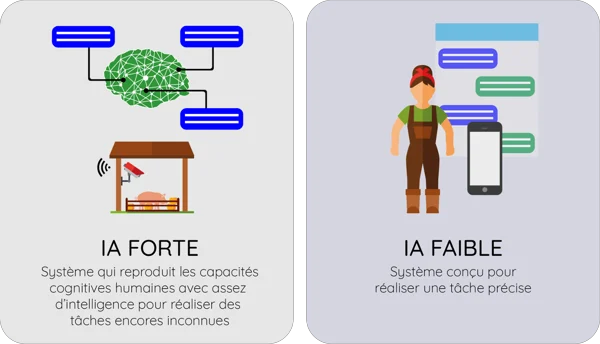
\includegraphics[width=0.8\linewidth]{chap1/images/IAFvsIAG.png}
    \caption{Weak AI vs.Strong AI}
    \label{fig:enter-label}
\end{figure}
\mySection{Machine Learning}{}

Machine Learning is an AI technology that aims to iteratively improve the performance of algorithms through data processing. In other words, Machine Learning allows computer systems to learn without being explicitly programmed for each task. Practically, this modern discipline allows for the discovery of patterns and predictions from data, relying on statistical methods, data mining, pattern recognition, and predictive analytics \cite{lebigdata2018}. Machine Learning is used in many fields such as speech recognition, fraud detection, consumer behavior prediction, and many more. Machine learning tasks are primarily organized into four categories: supervised learning, unsupervised learning, semi-supervised learning, and reinforcement learning.\\

\begin{figure}[ht!]
	\centering
	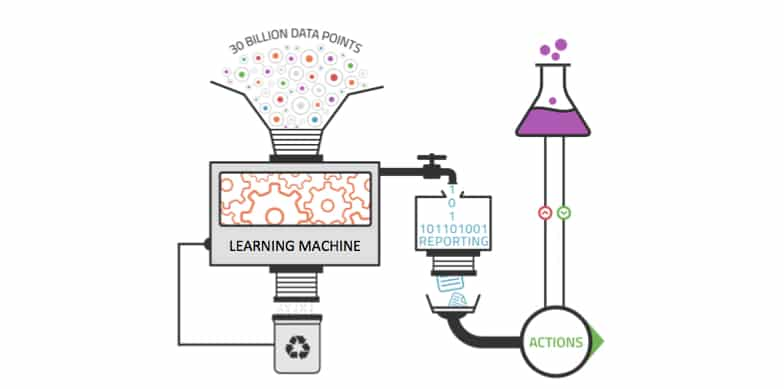
\includegraphics[width=0.8\linewidth]{Chap1/images/Marchinelearning2}
	\caption{Applications of Machine Learning \cite{lebigdata2018}.}
	\label{fig:marchinelearning2}
\end{figure}

\mySubSection{Supervised Learning}{}

Supervised learning is one of the most commonly used methods in the field of Machine Learning. It is a learning framework where an algorithm is trained on a labeled dataset. Each training example consists of an input and the corresponding output, allowing the algorithm to make predictions or classifications on new data based on the knowledge acquired during training, as shown in Figure \ref{MarchinelearningSupervise}. Supervised learning requires algorithms to train on a labeled dataset, and the goal is to map new input data to the desired target output value \cite{miraftabzadeh2019}.\\

\begin{figure}[ht!]
	\centering
	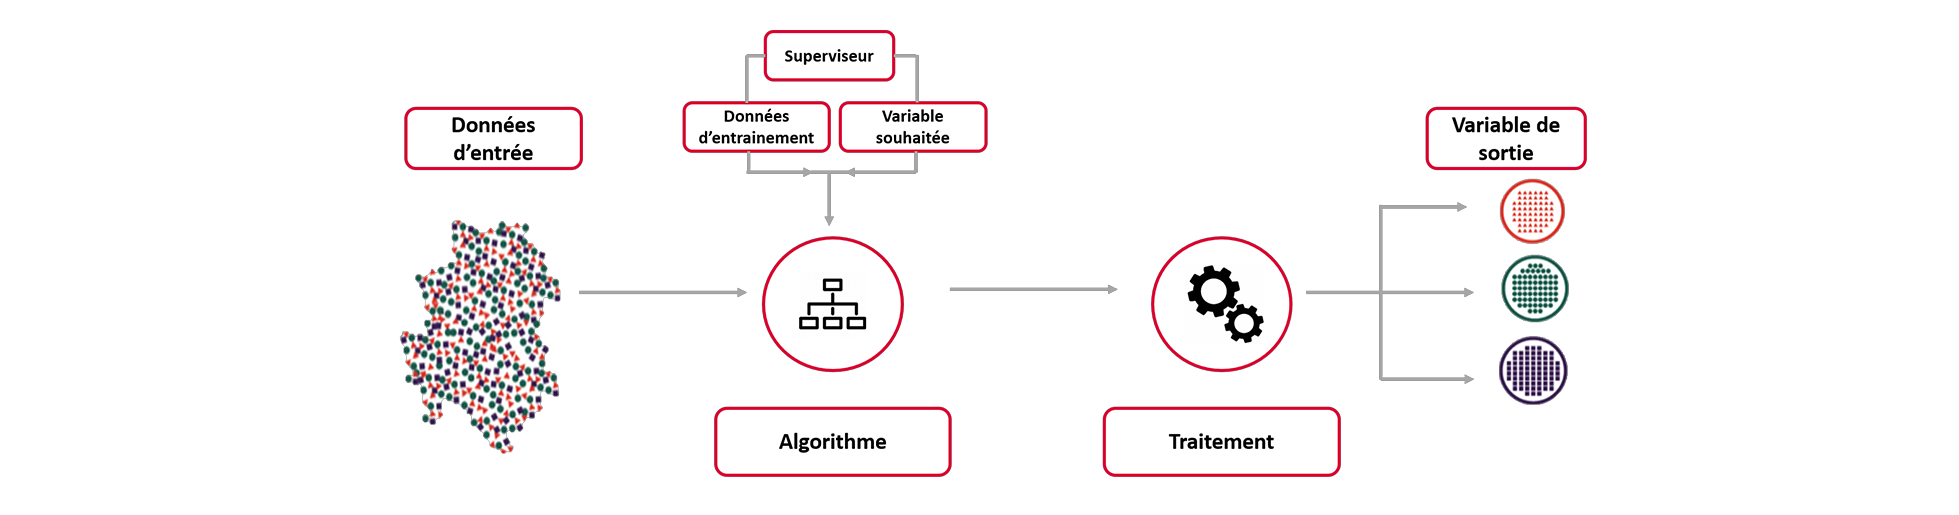
\includegraphics[scale=0.3]{Chap1/images/MarchinelearningSupervise}
	\caption{Supervised Learning \cite{Armandine2022}.}
	\label{MarchinelearningSupervise}
\end{figure}

Mathematically, problems in this type of learning are generally defined or formatted as follows: from a set of \( n \) observations \(\{\vec{x}1, \vec{x}_2, \ldots, \vec{x}_n\} = \{\vec{x}_i\}{i=1,\ldots,n}\) belonging to the set \(X\), and their labels \(\{y_1, y_2, \ldots, y_n\} = \{y_i\}_{i=1,\ldots,n}\) described in a set \(Y\), we aim to estimate the dependencies between the set \(X\) and \(Y\) to derive a model defined by a function \(y_i = f(\vec{x}_i) + \varepsilon_i\), where \(\varepsilon_i\) is a random noise. The algorithm, once trained with the provided labeled data, becomes capable of predicting labels on new unlabeled data.\\

\begin{figure}[ht!]
	\centering
	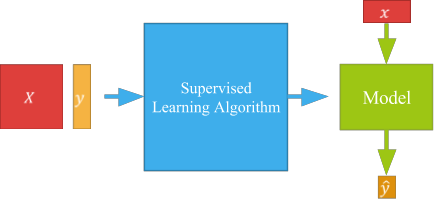
\includegraphics[scale=0.8]{Chap1/images/supervise.png}
	\caption{Supervised Learning}
	\label{fig:regressionvsclassification}
\end{figure}

In machine learning, the problems addressed are generally of two types: \textbf{Regression problems} and \textbf{Classification problems}.
\begin{enumerate}
	\item \textbf{Regression Problems:} These involve predicting continuous or real values based on input variables.
	\item \textbf{Classification Problems:} This involves predicting a discrete output variable, often called class labels, from a set of input data.
\end{enumerate}

\begin{figure}[ht!]
    \centering
    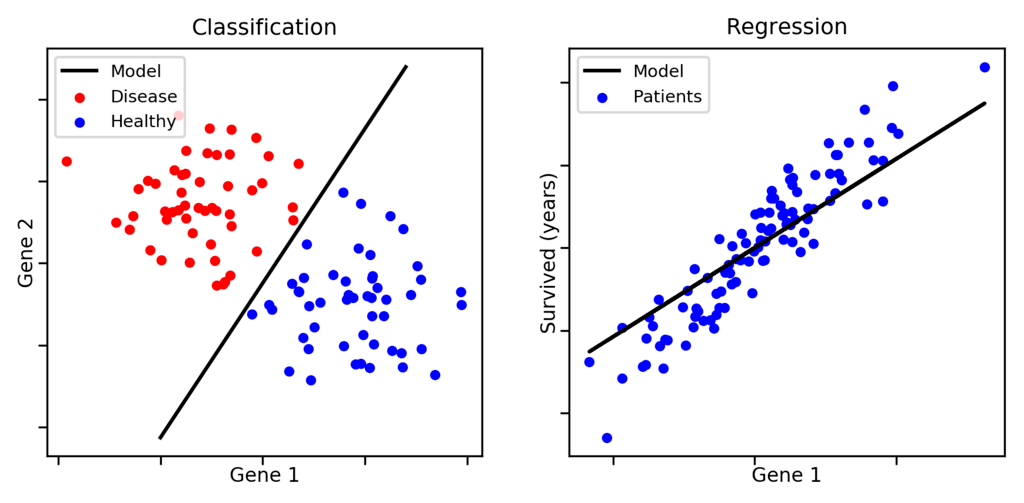
\includegraphics[width=0.6\linewidth]{chap1/images/regressionVSclassification.png}
    \caption{regression Vs.classification\cite{tensorflow2023}}
    \label{fig:enter-label}
\end{figure}

Over time, several algorithms have been developed to address the various problems of supervised learning. Among the main ones are:

\begin{itemize}
	\item \textbf{Linear Regression:} Used to predict the value of a dependent variable based on an independent variable . For example, predicting annual sales based on the education level or experience of a salesperson.

\begin{figure}[ht!]
    \centering
    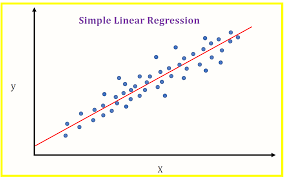
\includegraphics[width=0.5\linewidth]{chap1/images/linear regression.png}
    \caption{linear regression\cite{scikit-learn2023}}
    \label{fig:enter-label}
\end{figure}

 
	\item \textbf{Logistic Regression:} Suitable when dependent variables are binary.{SVM} is a relevant alternative when dependent variables are more difficult to classify.

    
 
	\item \textbf{Decision Trees:} Allow recommendations based on decision rules derived from classified data. For example, recommending a football team to bet on based on data like players' ages or the team's win percentage.






\item \textbf{Random Forest:} A collection of decision trees, where each tree is based on a bootstrap sample \cite{ho1998random}. The judgment is obtained by majority vote (classification) or by averaging results (regression).


 \begin{figure}[ht!]
     \centering
     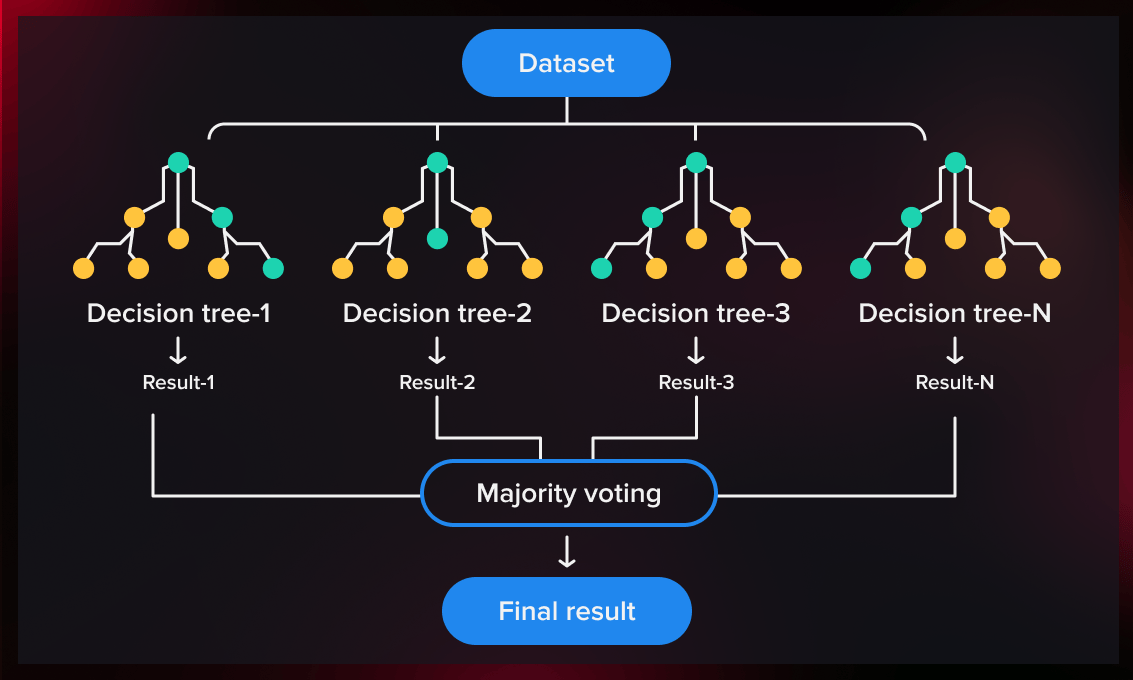
\includegraphics[width=0.5\linewidth]{chap1/images/randomforest.png}
     \caption{random forest\cite{ho1998random}}
     \label{fig:enter-label}
 \end{figure}

 
	\item \textbf{{SVM}:} Used for classification or regression. It uses a technique called the kernel trick to transform data and find an optimal boundary between possible outputs \cite{cortes1995support}.



 
	\item \textbf{Neural Networks:} Generally performed using a computer, reproducing or predicting the behavior of processes based on the factors that determine them.


 \begin{figure}[ht!]
     \centering
     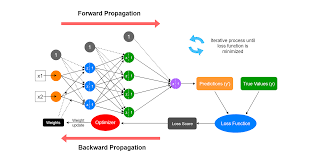
\includegraphics[width=0.5\linewidth]{chap1/images/neural network.png}
     \caption{neural network\cite{neuralnetwork2023}}
     \label{fig:enter-label}
 \end{figure}
	\item \textbf{{KNN}:} A classification algorithm that uses the similarity of neighboring data points to predict the class label of a new sample.


 \begin{figure}[ht!]
     \centering
     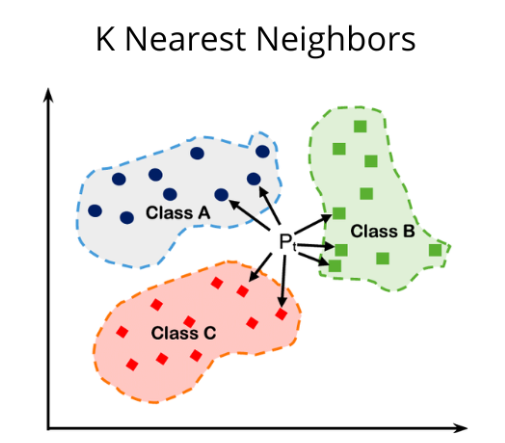
\includegraphics[width=0.5\linewidth]{chap1/images/knn.png}
     \caption{knn\cite{knn2023}}
     \label{fig:enter-label}
 \end{figure}
\end{itemize}

\mySubSection{Unsupervised Learning}{}

Unsupervised learning explores data without corresponding output variables, allowing it to discover the underlying structure or distribution of the data. Unlike supervised learning, where algorithms are guided by correct answers, unsupervised learning operates autonomously, seeking to identify patterns and intrinsic structures in the data \cite{ismaili2019}. The two main categories of algorithms in unsupervised learning are clustering and association. Clustering aims to divide a dataset into homogeneous groups, while association seeks to discover interesting relationships between variables in large databases.

\begin{figure}[ht!]
	\centering
	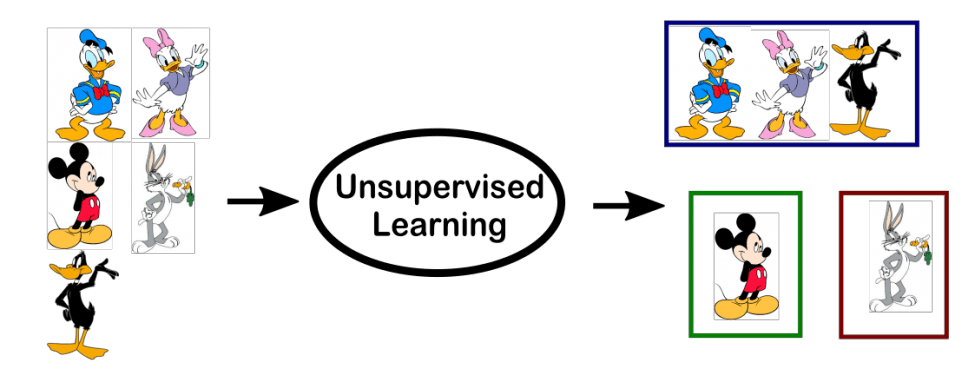
\includegraphics[scale=0.6]{Chap1/images/regressionVSclassification2}
	\caption{Unsupervised Learning \cite{ismaili2019}}
	\label{fig:regressionVSclassification2}
\end{figure}

In this subfield, several algorithms are commonly used:
\begin{itemize}
	\item \textbf{K-means Clustering:} It is an unsupervised learning algorithm used to solve clustering problems. K-means groups similar data points into clusters based on their characteristics or similarities \cite{pelleg1999accelerating}.
	\item \textbf{Association Rules:} These algorithms identify frequent relationships and associations between variables in datasets \cite{kamsu2013mining}.
	\item \textbf{Dimensionality Reduction:} This technique reduces the number of variables or features in a dataset while preserving relevant information. PCA is one of the popular methods for dimensionality reduction \cite{pelleg1999accelerating}.
\end{itemize}

\mySubSection{Semi-supervised Learning}{}

In machine learning, problems involving a large amount of input data (X = \(\{\vec{x}_1, \vec{x}_2, \ldots, \vec{x}_n\}\)) with only a few labeled data (Y = \(\{\vec{y}_1, \vec{y}_2, \ldots, \vec{y}_n\}\)) are called semi-supervised learning problems \cite{ismaili2019}. These problems lie between supervised learning, where all data is labeled, and unsupervised learning, where no labels are available.
A concrete example of a semi-supervised problem would be an archive of photos where only a few images are labeled (e.g., dog, cat, person) while most are not. In many real cases, labeling all data can be time-consuming or expensive, often requiring the expertise of domain specialists. Consequently, unlabeled data are often easier to collect and store.
To address semi-supervised problems, various techniques can be used. For example, unsupervised learning methods can be applied to discover and learn the underlying structure of input variables \cite{song2014semi}.
\mySubSection{Reinforcement Learning}{}
Reinforcement learning is a form of machine learning that focuses on training an algorithm to make decisions based on the rewards and punishments it receives. Unlike other methods where input-output pairs are provided, in reinforcement learning, we describe the current state of the system, specify a goal, provide a list of allowed actions with their environmental constraints, and then let the machine learning model experiment with achieving the goal on its own. This model uses the trial-and-error principle to maximize a reward \cite{zschech2021machine}.

\begin{figure}[ht!]
	\centering
	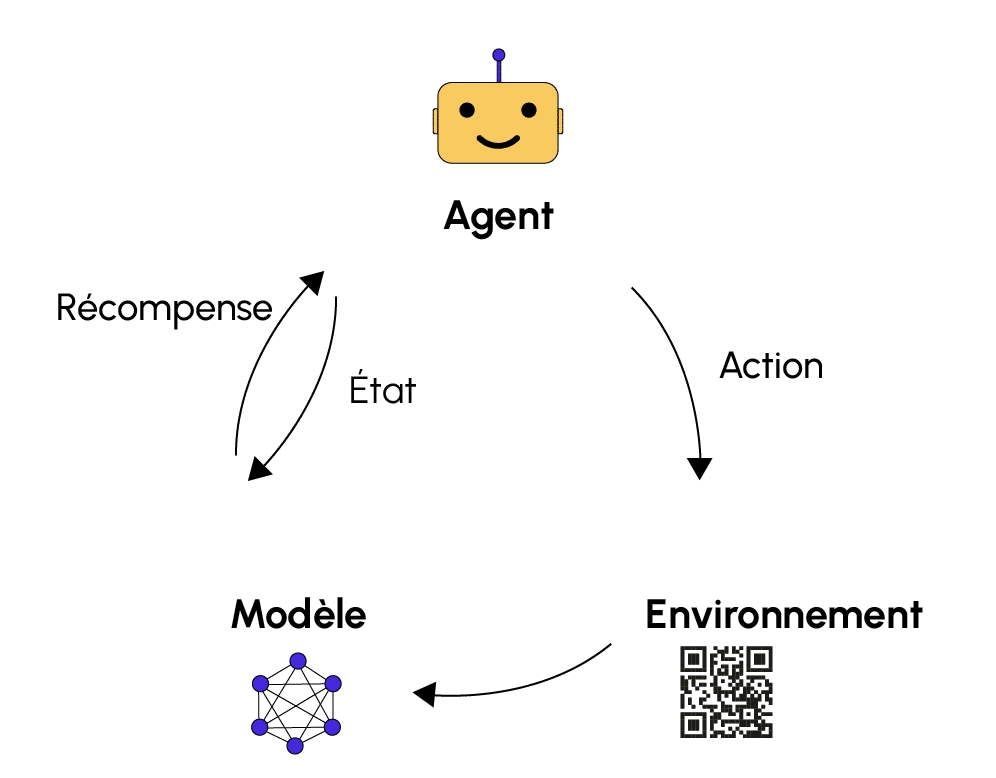
\includegraphics[scale=0.6]{Chap1/images/renforcement3}
	\caption{Reinforcement learning \cite{ismaili2019}}
	\label{fig:renforcement3}
\end{figure}

Reinforcement learning, as illustrated in Figure \ref{fig:renforcement3}, involves the use of several essential concepts and metrics, among which the main ones are as follows:

\begin{itemize}
	\item \textbf{Agent}: a system or robot that interacts and acts in the environment.
	\item \textbf{Action \( a \)}: an action selected from the set of possible actions.
	\item \textbf{State \( s \)}: a particular situation in which the agent finds itself.
	\item \textbf{Reward \( r(s,a) \)}: a positive or negative gain obtained by performing action \( a \) in state \( s \). The goal is to maximize the total benefits of a policy.
\end{itemize}


\mySection{Data Mining}{}
With the advent of artificial intelligence, the value of data has become crucial. Their diversity and rapid accumulation have resulted in an impressive mass of data requiring thorough analysis to be fully utilized. In this context, the implementation of analysis tools capable of extracting relevant information from these data is of paramount importance for data analysis professionals. For several decades, data mining has been the preferred method. This approach aims to search for and extract useful and unknown information from large sets of data stored in databases or data warehouses. The emergence of data mining in the 1990s was facilitated by technological advances that improved the computing power of computers. Data mining tools offer powerful statistical, mathematical, and analytical capabilities, aiming to analyze large datasets to identify trends, patterns, and relationships, to make informed decisions and plan effectively.

\mySubSection{Data Mining Process and Operation}{}

Data mining is generally carried out by data scientists and other professionals specializing in data analysis. However, it can also be undertaken by business analysts and personnel with a solid understanding of data, acting as data scientists within the organization. The essential elements of this exploration include machine learning, statistical analysis, as well as data management tasks necessary to prepare the data for analysis. The use of artificial intelligence (AI) tools has automated much of this process and simplified the exploration of massive datasets, such as customer databases or transaction records. The data mining process can be broken down into five steps, as illustrated in the following figure (Figure \ref{fig:datami}).

\begin{figure}[ht!]
	\centering
	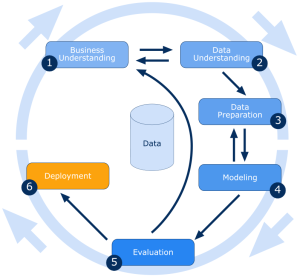
\includegraphics[scale=0.9]{Chap1/images/DataMi1}
	\caption{Data Mining Process \cite{kumar2023different}}
	\label{fig:datami}
\end{figure}

\begin{enumerate}
	\item \textbf{Understanding the Problem:} Before any data is touched, extracted, cleaned, or analyzed, it is important to understand the underlying entity and the ongoing project. It is also crucial to define the objectives to be achieved for problem resolution.
	
	\item \textbf{Data Collection:} This phase involves collecting the data that will be subjected to analysis. These data may be located in various source systems, such as data warehouses, which are increasingly used in big data environments. Data are also gathered from multiple external sources. These storage locations contain a mix of structured data (e.g., database tables) and unstructured data (e.g., text documents, images, videos). Regardless of the origin of the data, a data scientist often moves them to a data warehouse for subsequent process steps.
	
	\item \textbf{Data Preparation:} This phase is one of the most crucial phases of the process. It involves performing a set of treatments on the data to make them usable. It begins with data exploration, profiling, and preprocessing, followed by data cleaning to correct errors and other data quality issues. These issues include duplicates in the data, inconsistencies, incomplete records, or obsolete formats.
	
	\item \textbf{Modeling:} After the data preparation phase comes the information extraction phase. This step involves selecting the appropriate data mining technique and implementing one or more algorithms to perform the mining. These algorithms are machine learning algorithms that will train on these data to make the prediction process faster.
	
	\item \textbf{Evaluation:} Once the information extraction models' training is complete, the performance of the data models is evaluated. The analysis results can be aggregated, interpreted, and presented to decision-makers who have been largely excluded from the data mining process until now. At this stage, organizations can choose to make decisions based on the results.
\end{enumerate}

\mySubSection{Data Mining Techniques}{}

Data mining uses a set of algorithms and various techniques to convert large volumes of data into useful information. Here are some of the most popular techniques:

\begin{itemize}
	\item \textbf{Association Rules:} This technique aims to discover patterns in the data. Association rules, in the form of "if...then" statements, identify relationships between data items. Support measures how frequently these relationships appear, while confidence evaluates their accuracy. Popular algorithms include Apriori and FP-Growth.
	
	\item \textbf{Clustering:} Used in the absence of information about the types of data objects, clustering aims to group similar data. Common algorithms include K-means and hierarchical classification.
	
	\item \textbf{Classification:} To classify data into different groups based on a target attribute, classifiers predict the target label for each record. Common techniques include decision trees, neural networks, k-nearest neighbors (K-Means), support vector machines (SVM), and Bayesian methods.
	
	\item \textbf{Regression:} To model the relationships between variables and predict continuous numerical values, regression uses algorithms such as linear regression, logistic regression, and polynomial regression.
\end{itemize}

These techniques are essential for extracting meaningful information from data and making informed decisions in many fields.

\mySubSection{Importance of Data Mining}{}

Data mining is an essential process in data science that enables engineers to better understand their datasets. This process is of crucial importance in data analysis across various fields for the following reasons:

\begin{itemize}
	\item \textbf{Decision Making from Large Amounts of Data:} Data mining allows for extracting knowledge and hidden patterns from data. It helps organizations make informed decisions based on factual information rather than assumptions or intuitions. This can lead to more effective and profitable decisions.
	
	\item \textbf{Detection of Patterns and Trends:} Data mining helps discover significant patterns, correlations, and trends in the data. These insights can help organizations identify opportunities, anticipate future behaviors, detect market changes, and take preventive or proactive measures.
	
	\item \textbf{Forecasting and Planning:} By analyzing historical data and identifying relationships between variables, data mining can be used to predict future outcomes and establish plans and strategies accordingly. This can be useful in inventory management, demand forecasting, financial planning, etc.
	
	\item \textbf{Segmentation and Targeting:} Data mining allows grouping individuals or objects based on their common characteristics. This enables organizations to better understand their customers, segment the market into homogeneous groups, tailor offers and marketing campaigns accordingly, and target advertisements more precisely.
	
	\item \textbf{Personalization and Recommendation:} Data mining helps build personalized recommendation systems by analyzing users' preferences, behaviors, and purchase histories. This enhances user experience by providing relevant recommendations and increasing conversion and retention rates.
\end{itemize}

\mySubSection{Applications of Data Mining}{}

Data mining can be applied to all sectors that generate data and wish to benefit from it. Indeed, access to data is the key element to answering several questions within a domain. Here are some examples of how data mining is used in specific industries:

\begin{itemize}
	\item \textbf{Healthcare:} For many years, the integration of data mining in healthcare has enabled doctors to benefit from more effective treatment methods using data extracted from clinical trials and patient studies. Hospitals and clinics can thus improve patient outcomes and safety while reducing costs and response times.
	
	\item \textbf{Media and Telecommunications:} Companies in the media and telecommunications sector have access to an enormous amount of data on consumer preferences, such as the shows they watch or the internet plans they subscribe to. With these data, these companies can tailor their programming to consumer tastes, region, or other relevant factors. They can even recommend content to consume, a practice mastered by companies like Orange Cameroon, MTN Cameroon, YouTube, etc.
	
	\item \textbf{Bioinformatics:} Data mining plays an important role in the field of bioinformatics. Indeed, it is used to extract and analyze information on sequences, molecules, and gene expression to understand the functioning of certain biological processes.
\end{itemize}
\mySection{Conclusion}{}
In this chapter, we explored the interaction between the Domain Name System (DNS) and Machine Learning (ML), highlighting how ML enhances DNS security and performance. DNS, essential for translating domain names into IP addresses, is vulnerable to various attacks. ML offers powerful tools to detect and mitigate these threats by analyzing patterns and predicting anomalies.Key benefits of integrating ML with DNS include improved threat detection, anomaly identification, predictive analytics, and operational efficiency. However, challenges such as data privacy and model interpretability must be addressed. Finally,combining ML with DNS significantly enhances cybersecurity, ensuring a more secure and reliable internet infrastructure. Continued research and development in this field promise to refine these techniques and further strengthen DNS security.













































\begin{comment}
\mySection{Machine learning-based techniques}{}

Machine learning is a branch of Artificial Intelligence (AI) that empowers systems to learn and improve automatically from experience without needing explicit programming. The focus of machine learning is on developing computer programs that can access data and learn autonomously.Machine learning can be divided into three primary categories: supervised learning, unsupervised learning, and reinforcement learning.\\




\begin{figure}[ht!]
    \centering
    \includegraphics[width=0.75\linewidth]{Capture d'écran 2024-06-11 131107.png}
    \caption{Relatioship between Artificial intelligence,Machine learning and Deep learning}
    \label{fig:enter-label}
\end{figure}






\subsection{Supervised machine learning}

Supervised machine learning involves training algorithms to make predictions or classify data based on labeled training data. In supervised learning, the algorithm is trained on a dataset with known outcomes, allowing it to generalize from the labeled examples to make predictions on new, unseen data.The fundamental components in supervised machine learning are:
\begin{itemize}
    \item \textbf{Input (X)}: The data used by the model to make predictions.
    \item \textbf{Output (Y)}: The correct label or outcome for each example in the training data.
    \item \textbf{Output (f)}: The function that the algorithm learns to map inputs to outputs. The goal is to find the best model that accurately predicts the correct output for new input data.
\end{itemize}
The general equation for a supervised learning model is:
\[ Y = f(X) + \text{error} \]
where "error" signifies the difference between the predicted and actual outputs.
This type of learning is termed supervised because the algorithm's learning process from the training dataset is akin to a teacher supervising the process. The algorithm iteratively makes predictions on the training data and is corrected by the teacher until it reaches an acceptable performance level. Supervised learning algorithms are further categorized into regression and classification algorithms.

\textbf{Classification}: Tasks where the goal is to predict a categorical outcome, such as whether an email is spam. Common algorithms include logistic regression, decision trees, and support vector machines.

\textbf{Regression}: Tasks where the goal is to predict a continuous outcome, such as house prices. Common algorithms include linear regression, decision trees, and neural networks.

Some common supervised learning algorithms include:
\begin{itemize}
    \item \textbf{Support Vector Machines (SVM)}: Used for both classification and regression tasks, finding the hyperplane that best separates the data into classes or predicts values.






    \begin{figure}[ht!]
        \centering
        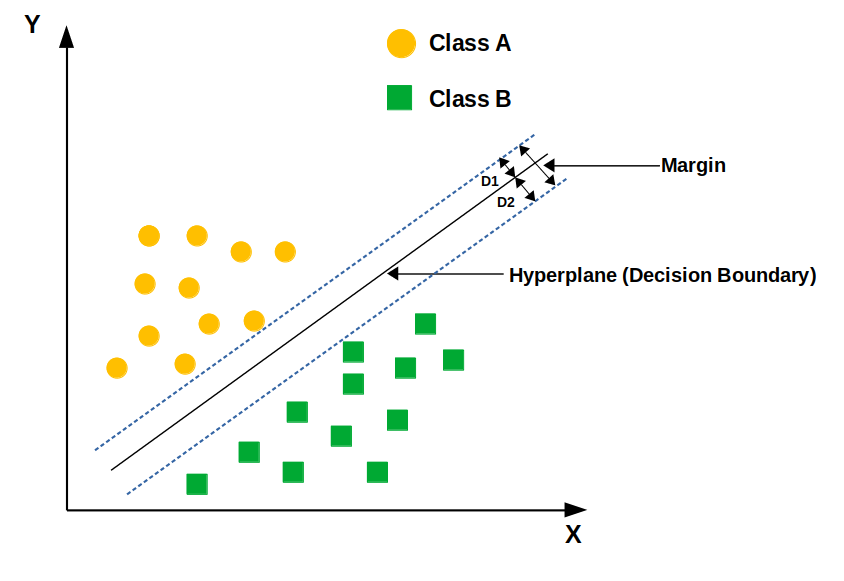
\includegraphics[width=0.5\linewidth]{svm.png}
        \caption{SVM}
        \label{FIGURE 2}
    \end{figure}


    
    \item \textbf{Neural Networks}: Used for diverse tasks like image recognition and speech recognition, consisting of interconnected nodes that learn from input data.



    \begin{figure}[ht!]
        \centering
        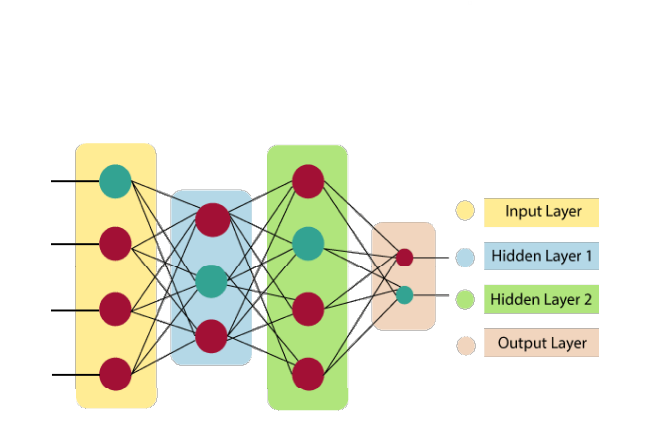
\includegraphics[width=0.5\linewidth]{rnn.png}
        \caption{Neural network}
    \end{figure}


    
    \item \textbf{Linear Regression}: Used for regression tasks, modeling the relationship between input and output variables using a linear function.

    \item \textbf{Logistic Regression}: Used for binary classification tasks, modeling the probability of outcomes using a logistic function.

\begin{figure}[ht!]
    \centering
    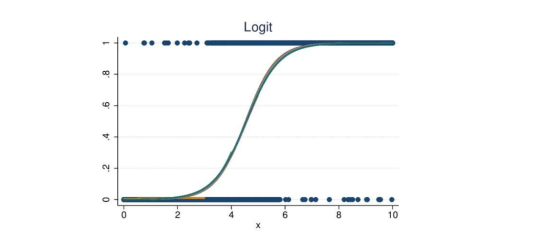
\includegraphics[width=0.5\linewidth]{logistic regrestion.png}
    \caption{logistic regression}
    \label{fig:enter-label}
\end{figure}


    
    \item \textbf{Decision Trees}: Used for both classification and regression tasks, creating a tree-like model of decisions.



    

\begin{figure}[ht!]
    \centering
    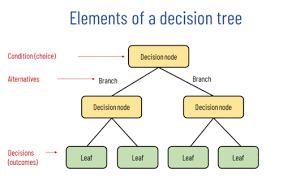
\includegraphics[width=0.3\linewidth]{decision tree.png}
    \caption{Decision tree}
    \label{fig:enter-label}
\end{figure}



    
    \item \textbf{Random Forest}: An extension of decision trees, combining multiple trees to improve accuracy and reduce over-fitting.
    \item \textbf{K-Nearest Neighbors (KNN)}: Used for classification, classifying new data points based on the K nearest neighbors in the training set.
\end{itemize}

\subsection{Unsupervised Machine Learning}

Unsupervised machine learning involves algorithms learning from unlabeled data. Unlike supervised learning, there is no target variable, and the algorithm seeks to find patterns and relationships in the data without predefined outputs. Unsupervised learning is useful for exploratory data analysis, detecting anomalies, clustering similar data points, and reducing data dimensionality.\\

Types of unsupervised learning algorithms include:
\begin{itemize}
    \item \textbf{Clustering}: Grouping similar data points based on feature similarity.
    \item \textbf{Dimensionality Reduction}: Reducing the number of features while preserving important information to simplify data analysis.
    \item \textbf{Association Rule Learning}: Finding relationships between variables in the data, identifying frequent co-occurrences of items.
\end{itemize}

Common unsupervised learning algorithms include:
\begin{itemize}
    \item \textbf{K-Means Algorithm}: Used for clustering.
    \item \textbf{Principal Component Analysis (PCA)}: Used for dimensionality reduction.
    \item \textbf{A priori Algorithm}: Used for association rule learning.
\end{itemize}

\subsection{Reinforcement Learning}

Reinforcement learning involves an agent learning to make decisions by interacting with an environment. The agent receives feedback as rewards or punishments based on its actions and learns to optimize its behavior to maximize rewards. Reinforcement learning is used in applications such as robotics, game playing, and autonomous vehicles.
At a high level, reinforcement learning can be formulated as a Markov decision process (MDP) consisting of:
\begin{itemize}
    \item \textbf{Environment}: The physical world in which the agent operates.
    \item \textbf{State}: The current situation of the agent.
    \item \textbf{Reward}: Feedback from the environment.
    \item \textbf{Policy}: The method to map an agent's state to actions.
    \item \textbf{Value}: The future reward an agent would receive by taking an action in a particular state.
\end{itemize}

\subsection{Federated Learning}

Federated learning is a decentralized machine learning approach that enables multiple parties to collaboratively train a model without sharing their data. Training data remains on the participants' devices, with only model updates being exchanged. This approach preserves data privacy and reduces communication costs.\\

Types of federated learning include:
\begin{itemize}
    \item \textbf{Horizontal Federated Learning}: Participants have the same features but different samples.
    \item \textbf{Vertical Federated Learning}: Participants have different features but the same samples.
\end{itemize}

\subsection{Deep Learning}

Deep learning, a subset of machine learning, involves training artificial neural networks with multiple layers to perform complex tasks such as image recognition, speech recognition, natural language processing, and autonomous driving. Unlike traditional machine learning algorithms that require manual feature engineering, deep learning algorithms can automatically learn high-level features from raw data, making them effective for tasks where relevant features are not well understood.

Neural networks consist of layers of interconnected nodes, called neurons, performing simple calculations on input data. The output of one layer serves as input to the next layer, allowing the network to learn increasingly complex data representations.
\mySection{Machine learning in DNS security}{}
DNS (Domain Name System) is a critical component of the internet infrastructure, responsible for translating human-readable domain names into IP addresses. As the internet continues to grow, DNS has become an increasingly attractive target for cyber attackers, who may attempt to exploit vulnerabilities in the system to launch various types of attacks, such as domain name hijacking, cache poisoning, and distributed denial-of-service (DDoS) attacks. ML has emerged as a powerful tool in the field of DNS security, enabling the detection and mitigation of these threats. ML algorithms can analyze large volumes of DNS traffic data, identify patterns and anomalies, and quickly detect and respond to potential attacks. This can greatly improve the overall security and reliability of the DNS system, protecting both individuals and organizations from the consequences of DNS-based attacks.
\subsection{Application of ML in cybersecurity}
In the rapidly evolving landscape of cybersecurity, the advent of machine learning (ML) has brought about a transformative shift in the way we approach the detection, prevention, and mitigation of cyber threats. As the volume, velocity, and complexity of cyber attacks continue to escalate, traditional rule-based security approaches have become increasingly inadequate. ML, with its ability to identify patterns, learn from data, and adapt to changing environments, has emerged as a powerful tool in the cybersecurity arsenal.
The application of ML in cybersecurity spans a wide range of domains, from network intrusion detection and malware analysis to user behavior analytics and predictive security intelligence. By leveraging the strengths of ML, security professionals can gain a deeper understanding of the evolving threat landscape, automate the detection and response processes, and ultimately enhance the overall resilience of their organizations.

\begin{enumerate}
\item Network Intrusion Detection and Prevention:

One of the most prominent applications of ML in cybersecurity is in the realm of network intrusion detection and prevention. Traditional rule-based intrusion detection systems (IDS) often struggle to keep up with the dynamic nature of cyber threats, as they rely on predefined signatures and patterns. ML-based IDS models, on the other hand, can learn from past network traffic and security events, enabling them to detect and mitigate novel and previously unknown attacks.These ML-powered IDS systems leverage a variety of techniques, such as supervised learning for anomaly detection, unsupervised learning for identifying suspicious activity patterns, and deep learning for complex pattern recognition. By continuously analyzing network traffic, these systems can detect and respond to anomalies in near real-time, significantly improving the organization's ability to defend against cyber threats.\cite{Meidan2018},proposed a  Network-based Detection of Botnet Attacks Using Deep Autoencoders in this domain.

\item Malware Analysis and Classification:

The rapid proliferation of malware, ranging from ransomware to advanced persistent threats (APTs), has also driven the application of ML in cybersecurity. Traditional static and dynamic analysis methods for malware detection can be time-consuming and often struggle to keep pace with the ever-evolving malware landscape. ML-based malware analysis and classification models can automate the process of identifying and categorizing malware samples. These models leverage techniques like supervised learning, deep learning, and reinforcement learning to analyze the characteristics of malware, such as its behavior, code structure, and network communication patterns. By continuously learning from new malware samples, these systems can improve their detection capabilities and quickly identify and mitigate emerging threats.\cite{Zichichi2021} proposed a comparative analysis on this.

\item User Behavior Analytics:

Another critical area where ML has found application in cybersecurity is user behavior analytics (UBA). Traditional security approaches often rely on rule-based systems to detect suspicious user activities, which can be limited in their ability to adapt to changing user behaviors and patterns. ML-based UBA models, on the other hand, can learn and analyze the normal patterns of user behavior, such as login patterns, access privileges, and data access activities. By establishing a baseline of normal user behavior, these models can then detect anomalies and identify potential insider threats or compromised user accounts. This proactive approach to user behavior monitoring can significantly enhance an organization's ability to detect and mitigate insider threats and account-based attacks.\cite{Siadati2017} proposed a technic based on topological features.

\item Predictive Security Intelligence

The application of ML in cybersecurity also extends to the realm of predictive security intelligence. By analyzing a vast array of security-related data, including threat intelligence, vulnerability information, and historical incident data, ML models can identify patterns, trends, and correlations that can help security teams anticipate and prepare for future threats.These predictive security intelligence models leverage techniques like supervised learning, unsupervised learning, and natural language processing to extract meaningful insights from unstructured data. This information can be used to prioritize risk, optimize security controls, and proactively allocate resources to address emerging threats before they can cause significant damage.
\end{enumerate}
\subsubsection{Challenges and considerations}

While the application of ML in cybersecurity holds tremendous promise, there are also a number of challenges and considerations that must be addressed:
\textbf{Data Availability and Quality:} Effective ML-based security solutions require high-quality, labeled data for training and validation. Obtaining comprehensive and representative security data can be a significant challenge, particularly in the face of evolving threats and increasing data privacy concerns.\\
\textbf{Model Interpretability and Explainability:} As ML models become more complex, the "black box" nature of these systems can make it difficult to understand the reasoning behind their decisions. Addressing the need for interpretable and explainable AI is crucial for building trust and ensuring the accountability of ML-based security solutions.\\
\textbf{Operational Scalability and Integration:} Deploying and maintaining ML-based security systems in a production environment requires careful consideration of scalability, real-time processing, and seamless integration with existing security infrastructure.\\
\textbf{Ethical Considerations and Regulatory Compliance:} The use of ML in cybersecurity raises important ethical considerations, such as data privacy, algorithmic bias, and the potential for unfair or discriminatory outcomes. Ensuring compliance with evolving data protection regulations is also a critical concern.
\subsection{Use cases in DNS}

\textbf{Malicious Domain Detection}

One of the primary use cases of ML in DNS is the detection of malicious domains. Traditional rule-based approaches to identifying malicious domains often struggle to keep pace with the rapidly changing tactics of cybercriminals. ML-based models, on the other hand, can analyze a vast amount of DNS data, including domain registration information, network traffic patterns, and historical reputation data, to accurately identify and flag suspicious domains.
These ML-powered detection systems leverage techniques like supervised learning, unsupervised learning, and deep learning to continuously learn from new data and improve their ability to detect even the most sophisticated domain-based threats, such as phishing, malware distribution, and command-and-control (C2) infrastructure.\\
\textbf{Anomaly Detection and DDoS Mitigation}
The DNS infrastructure is also vulnerable to various types of attacks, including Distributed Denial of Service (DDoS) attacks, which can overwhelm the system and disrupt critical online services. ML-based anomaly detection models can analyze DNS traffic patterns and server performance metrics to identify and mitigate such attacks in near real-time.

These models can learn the normal behavior of DNS traffic and quickly detect deviations that may indicate a DDoS attack or other anomalous activity. By leveraging techniques like clustering, outlier detection, and time-series analysis, ML-based anomaly detection systems can help security teams respond more effectively to DNS-based attacks and ensure the availability and reliability of the DNS infrastructure.

\textbf{Predictive Domain Lifecycle Management}

Another application of ML in the DNS domain is predictive domain lifecycle management. ML models can analyze a vast amount of domain registration data, including factors like domain age, registrant information, and historical registration patterns, to predict the likelihood of a domain being used for malicious purposes.

By identifying potentially risky domains early in their lifecycle, security teams can take proactive measures to mitigate the associated threats, such as monitoring the domain, blocking its resolution, or collaborating with domain registrars to suspend the registration. This predictive approach to domain lifecycle management can significantly enhance an organization's ability to stay ahead of emerging domain-based threats.

\textbf{Optimizing DNS Performance and Availability}

ML-based models can also be used to optimize the performance and availability of the DNS infrastructure. By analyzing DNS server metrics, network traffic patterns, and user behavior data, these models can help identify bottlenecks, optimize load balancing, and predict potential service disruptions.

This can include techniques like workload forecasting, resource allocation optimization, and proactive maintenance scheduling. By leveraging the insights generated by ML, DNS administrators can ensure that the DNS infrastructure remains resilient, responsive, and able to handle the ever-increasing demands placed on it.

\textbf{Challenges and Considerations}

While the application of ML in the DNS domain holds substantial promise, there are also several challenges and considerations that must be addressed:\\

\textbf{Data Availability and Privacy:} Effective ML-based DNS security solutions require access to a vast amount of DNS data, which can raise concerns about data privacy and regulatory compliance.\\
\textbf{Model Interpretability:} As with other domains, the interpretability and explainability of ML models used in DNS security are crucial for building trust and ensuring accountability.\\
\textbf{Operational Integration:} Integrating ML-based DNS security solutions into existing infrastructure and workflows can be a complex and resource-intensive process, requiring careful planning and implementation.
\textbf{Continuously Evolving Threats:} The threat landscape in the DNS domain is constantly evolving, necessitating the ongoing adaptation and retraining of ML models to maintain their effectiveness.

\mySection{Conclusion}{}
In this chapter, we explored the synergy between the Domain Name System (DNS) and Machine Learning (ML), highlighting how ML enhances DNS security and performance. DNS, essential for translating domain names into IP addresses, is vulnerable to various attacks. ML offers powerful tools to detect and mitigate these threats by analyzing patterns and predicting anomalies.

Key benefits of integrating ML with DNS include improved threat detection, anomaly identification, predictive analytics, and operational efficiency. However, challenges such as data privacy and model interpretability must be addressed.

Overall, combining ML with DNS significantly enhances cybersecurity, ensuring a more secure and reliable internet infrastructure. Continued research and development in this field promise to refine these techniques and further strengthen DNS security.
%\label{chapEtatDeLart}
%\myMinitoc{Profondeur de la minitoc (section|subsection|subsubsection)}{Titre de la minitoc}
%\\myMiniToc{section}{Sommaire}
\myCleanStarChapterEnd




\end{comment}